\documentclass[11pt, a4wide]{article}

\usepackage{polski}
\usepackage{a4wide}
\usepackage[utf8]{inputenc}
\usepackage{hyperref}

\usepackage{amssymb}
\usepackage{amsmath}
\usepackage{algorithmicx}
\usepackage{algorithm}
\usepackage{graphicx}
\usepackage{epstopdf}
\usepackage{algpseudocode}
\usepackage{float}


\title{Algorytm ewolucyjny dla problemu flow shop}
\author{Jan Sochiera \and Krzysztof Chrobak}

\begin{document}
\maketitle
\tableofcontents

\section{Problem}
\subsection{Definicja}
Problem flow shop jest NP-trudną odmianą problemu szeregowania $n$ zadań na $m$ maszynach, w której:
\begin{itemize}
  \item każde zadanie musi zostać wykonane na każdej maszynie
  \item kolejność wykonywania zadań na wszystkich maszynach jest taka sama
  \item zadanie może być wykonywane jednocześnie na tylko jednej maszynie
\end{itemize}
Ten abstrakcyjny opis pasuje do wielu rzeczywistych zagadnień, np. linii montażowej w 
fabryce, na której przetwarzane przedmioty przechodzą przez poszczególne etapy produkcji w tej
samej kolejności, choć czas który w nich spędzają może się znacząco różnić.

Problem jest w całości definiowany przez następujące dane:
\begin{itemize}
  \item $n$ - ilość zadań
  \item $m$ - ilość maszyn 
  \item macierz $T$, w której $T_{ij}$ to czas przetwarzania $j$-tego zadania na $i$-tej maszynie
\end{itemize}

\subsection{Przestrzeń przeszukiwania}
Łatwo zauważyć, że przebieg całego procesu odpowiadającego danej instancji problemu flow shop
jest w całości zdefiniowany przez kolejność zadań na pierwszej maszynie, ponieważ na każdej innej
zadania będą wykonywane dokładnie w tym samym porządku. Wynika ztąd, że przestrzenią poszukiwań jest
$S_n$ : zbiór wszystkich permutacji zbioru $n$-elementowego. Oczywiście $|S_n| = n!$, więc dla $n>10$
przeszukanie całej przestrzeni staje się niepraktyczne.

\subsection{Funkcja celu}
W naszym projekcie przyjęliśmy, że funkcją celu będzie  $ makespan : S_n \rightarrow \mathbb{R} $, który
definiujemy jako czas od rozpoczęcia wykonywania pierwszego zadania na pierwszej maszynie do 
zakończenia wykonywania ostatniego zadania na ostatniej maszynie.

\subsection{Rozkład wartości $makespan(\pi)$}
Dla instancji problemu, gdzie $n$ jest duże przestrzeń przeszukiwań jest tak ogromna, że trudno
cokolwiek powiedzieć o rozkładzie wartości $makespan$, dlatego postanowiliśmy sprawdzić jak ta funkcja
zachowuje się dla $n = 10$, gdzie możliwe jest policzenie jej wartości dla każdego $\pi \in S_n$.
W naszym eksperymencie przyjęliśmy $m = TODO$, a $T_{ij}$ wylosowaliśmy z rozkładem jednostajnym 
z przedziału $[10, 20]$. Jakość rozwiązania $Q$ definiujemy jako:
$$ Q(\pi) = \frac{makespan(\pi)}{makespan(\pi_{opt})}$$
gdzie $\pi_{opt}$ to optymalne szeregowanie zadań dla tej instancji.

Na wykresie \ref{rozklad} można zobaczyć histogram dla $Q$. Na wykresie \ref{dystrybuanta} znajduje 
się logarytmiczny wykres "dystrybuanty" (\% populacji o wartości $Q$ mniejszej niż ta na osi $x$) tej 
wartości. Widać na nim, że wraz ze spadkiem $Q$ drastycznie maleje ilość osobników, dla których $makespan$
przyjmuje właśnie takie wartości.


\begin{figure}[H]
\caption{Rozkład $Q$}
\label{rozklad}
\begin{center}
  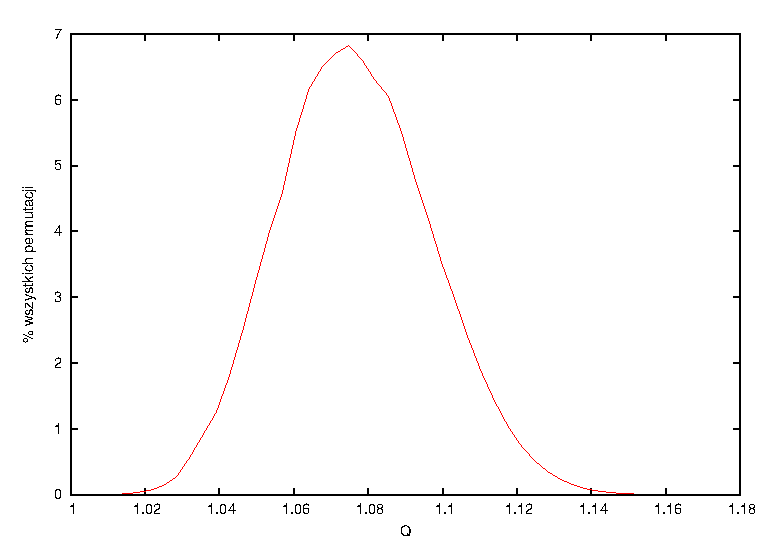
\includegraphics{histogram.eps}
\end{center}
\end{figure}

\begin{figure}[H]
\caption{Dystrybuanta $Q$}
\label{dystrybuanta}
\begin{center}
  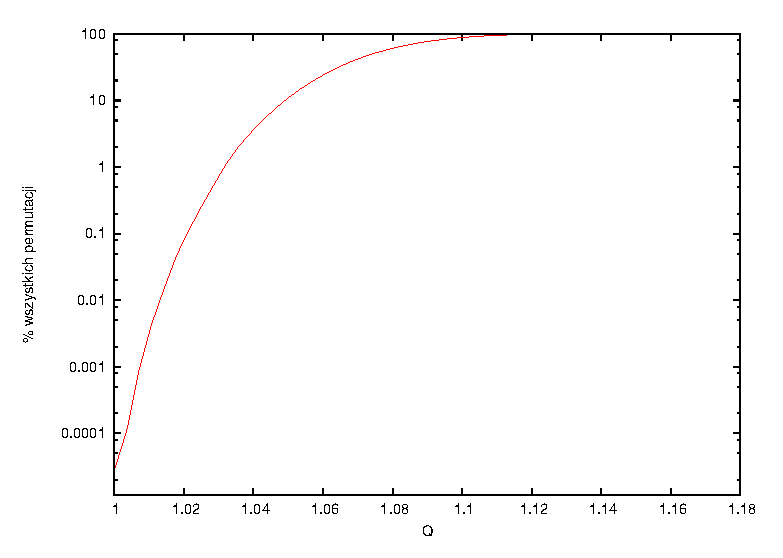
\includegraphics{dystrybuanta.eps}
\end{center}
\end{figure}




\section{Algorytm}
Algorytm który zaimplementowaliśmy jest modyfikacją klasycznego SGA, do której dodaliśmy przeszukiwanie lokalne
i zwiększanie różnorodności populacji poprzez dodawanie losowych imigrantów. Dane wejściowe dla tego algorytmu:
\begin{description}
  \item[instance] instancja problemu flow shop
  \item[population\_size] rozmiar populacji
  \item[num\_parents] ilość rodziców
  \item[mutation\_probability] prawdopodobieństwo mutacji
  \item[$\alpha$] parametr imigracji
\end{description}
Pseudokod algorytmu znajduje się na listingu~\ref{algorytm}

\begin{algorithm}[H]
\caption{Algorytm ewolucyjny dla problemu flow shop}
\label{algorytm}
\begin{algorithmic}
  \State $P \gets RandomPopulation(population\_size)$
  \State $EvaluatePopulation(P, instance)$
  \While{not $TerminationCondition(P)$}
    \State $Parents \gets SelectParents(P, num\_parents)$ 
    \State $Children \gets Crossover(Parents)$
    \State $Children \gets Mutate(Children, mutation\_probability)$
    \State $Children \gets LocalSearch(Children, instance)$
    \State $Population \gets Replace(Population, Children)$
    \State $Population \gets AddImigrants(Population, instance, \alpha)$
  \EndWhile
\end{algorithmic}
\end{algorithm}

\subsection{Ocena osobników $EvaluatePopulation$}
Pojedynczego osobnika można ocenić przy pomocy prostego algorytmu dynamicznego, korzystającego
z następujących zależności ($E[i,j]$ to czas zakończenia wykonywania $j$-tego w kolejności zadania
na $i$-tej maszynie, przy kolejności zadań $\pi$):
$$ E[1, 1] = t_{1,\pi(1)} $$
$$ E[1, i] = E[1, i-1] + t_{1,\pi(i)}\ \  i = 2 \ldots n$$
$$ E[i, 1] = E[i-1, 1] + t_{i,\pi(1)}\ \  i = 2 \ldots m$$
$$ E[i, j] = max(E[i-1, j], E[i, j-1]) + t_{i, \pi(j)} \ \ i = 2 \ldots n \ \ j = 2 \ldots m $$
Algorytm dynamiczny oceny jednego osobnika ma złożoność $O(nm)$

\subsection{Warunek zakończenia $TerminationCondition$}
Nasz algorytm kończy działanie gdy przekroczy ustaloną z góry ilość iteracji pętli while, albo
gdy uda mu się osiągnąć wartość funkcji celu znaną jako optymalna dla danego problemu. Oczywiście
ten ostatni warunek należałoby usunąć chcąc rozwiązywać nowe problemy, ale podczas testowania 
algorytmu szukanie rozwiązania lepszego niż optymalne nie miało żadnego sensu.

\subsection{Wybór rodziców $SelectParents$}
Eksperymentowaliśmy z dwiema metodami wyboru rodziców:
\begin{itemize}
  \item Metoda ruletki z różnymi skalowaniami funkcji przystosowania
  \item Metoda k-najlepszych osobników
\end{itemize}
W ostatecznej wersji algorytmu zdecydowaliśmy się na drugą metodę, ponieważ
w połączeniu z metodą ruletki nie dało się stosować wybranej przez nas strategii zastępowania. Okazało 
się również, że warto pozwalać wszystkim osobnikom wziąć udział w reprodukcji.

\subsection{Krzyżowanie $Crossover$}
Osobniki wybrane do reprodukcji są losowo kojarzone w pary, tak że każdy ma dokładnie jednego partnera.
Do krzyżowania użyliśmy prostego operatora PMX.

\subsection{Mutacja $Mutate$}
Z pewnym małym prawdopodobieństwem (po kilku eksperymentach ustaliliśmy tą wartość na 5\%) każde dziecko jest
mutowane. Mutacja polega na złożeniu permutacji osobnika z losową permutacją o około 75\% punktów stałych.

\subsection{Przeszukiwanie lokalne $LocalSearch$}
Ten krok algorytmu ma kluczowe znaczenie dla jakości otrzymywanych rozwiązań, ponieważ jeśli za bardzo przyspieszy
zbieżność, to algorytm będzie miał tendencję do utykania w minimach lokalnych, a jeśli będzie go brakowało, 
to ewolucja nie będzie w stanie w rozsądnym czasie znaleźć dobrego rozwiązania. Czas obliczania tego kroku
decyduje też o czasie działania całego algorytmu, bo polega on na przeszukaniu pewnego otoczenia osobnika
w poszukiwaniu lepszego niż on sam sąsiada. Zdecydowaliśmy się na następujący schemat przeszukiwania lokalnego:
\begin{algorithm}[H]
\caption{Przeszukiwanie lokalne}
\label{localsearch}
\begin{algorithmic}
  \For {$i \gets 1 \ldots |Children|$}
    \State $I \gets Children[i]$
    \State $best \gets I$
    \State $mspan \gets makespan(I)$
    \For {$j \gets 1 \ldots n$}
      \For {$k \gets 1 \ldots n$}
        \State $Candidate \gets insert(I, i, k)$
        \State $cspan \gets makespan(Candidate)$
        \If{$cspan < mspan $}
          \State $mspan \gets cspan$
          \State $best \gets Candidate$
        \EndIf
      \EndFor
    \EndFor
    \State $Children[i] = best$
  \EndFor
\end{algorithmic}
\end{algorithm}
Czyli mówiąc krótko dla każdego dziecka próbujemy włożyć $j$-te zadanie na $k$-tą pozycję dla 
wszystkich sensownych $j$ i $k$. Złożoność obliczeniowa takiego podejścia przy zastosowaniu algorytmu
oceny przytoczonego wcześniej to $O(mn^3|Children|)$, ale przy zastosowaniu sprytniejszego algorytmu
z pracy \cite{tai90}, można ją zredukować do $O(mn^2|Children|)$.

\subsection{Zastępowanie $Replace$}
Aby uniemożliwić najlepszym osobnikom zdominowanie populacji po kilku iteracjach, użyliśmy schematu
zastępowania, który bierze pod uwagę tylko czwórkę osobników : parę rodziców i ich dzieci. Z takiej
czwórki wybieramy 2 najlepszych osobników, i to oni przechodzą do następnego pokolenia. Oczywiście
tą procedurę należy powtórzyć dla wszystkich par rodziców wygenerowanych w kroku krzyżowania.

\subsection{Imigracja $AddImigrants$}
Aby algorytm działał dowolnie długo, postanowiliśmy mierzyć różnorodność osobników w populacji i w razie jej
spadku zastępować najgorsze osobniki losowymi. Wprowadziliśmy współczynnik różnorodności $D$:
$$ D = \frac{\text{ilość różnych osobników}}{\text{ilość osobników}} $$
Ilość osobników zastępowanych losowymi jest określona przez parametr $\alpha$ i zależność:
$$ N_{random} = \lfloor \alpha * (1 - D) * population\_size  \rfloor $$
Aby nowe osobniki nie zostały wyeliminowane po jednej iteracji, wykonujemy dla każdego z nich przeszukiwanie
lokalne.




\section{Implementacja}
Algorytm zaimplementowaliśmy w C++ przy użyciu biblioteki OpenMP, która umożliwiła nam łatwe zrównoleglenie
przeszukiwania lokalnego (ten proces jest niezależny dla każdego osobnika).

\subsection{Kompilacja}
Potrzebne programy:
\begin{itemize}
  \item Kompilator obsługujący OpenMP, np. GCC 4.7
  \item CMake
\end{itemize}
Polecenia do skompilowania załączonego programu:
\begin{enumerate}
  \item \verb|tar -xvf flowshop.tar|
  \item \verb|cd flowshop/program|
  \item \verb|mkdir build|
  \item \verb|cd build|
  \item \verb|cmake .. -DCMAKE_BUILD_TYPE=Release|
  \item \verb|make|
\end{enumerate}
Jeśli kompilacja przebiegnie pomyślnie, wygenerowany zostanie program \verb|flowshop|. Po uruchomieniu
bez żadnych opcji wyświetli krótką instrukcję obsługi.





\section{Wyniki}
\subsection{Parametry algorytmu}

\begin{table}[H]
\caption{Wartości parametrów algorytmu}
\label{parametry}
\begin{center}
\begin{tabular}{|l|l|}
  \hline
  parametr & wartość \\
  \hline
  rozmiar populacji & 1000 \\
  ilość rodziców & 1000 \\
  prawdopodobieństwo mutacji & 0.05 \\
  $\alpha$ & 0.3 \\
  \hline
\end{tabular}
\end{center}
\end{table}


\subsection{Jakość rozwiązań}
TODO

\subsection{Działanie algorytmu}
W każdej iteracji algorytmu zapisywaliśmy średnią wartość funkcji $makespan$ dla całej populacji
oraz dla najlepszego osobnika. Wykres \ref{progress} przedstawia jak zmieniają się te wartości 
podczas jednego uruchomienia algorytmu dla trudnego problemu ($m = 20$, $n = 500$). Widać na nim
że mimo że postęp jest coraz wolniejszy, to algorytm nie pozwala by średnia wartość stała się równa
najlepszej, tym samym zabezpieczając populację przed staniem się zbiorem kopii jednego osobnika.

Poniższy wykres \ref{diversity} przedstawia wartość współczynnika różnorodności w zależności od numeru iteracji.
Widać na nim, że algorytm stara się utrzymać możliwie wysoką wartość tego wskaźnika, lecz z czasem
wylosowanie osobnika, który różnił by się od wszystkich istniejących i jednocześnie miał na tyle
dobrą wartość funkcji $makespan$, by przetrwać proces selekcji jest coraz trudniejsze.

\begin{figure}[H]
\caption{Przebieg działania algorytmu}
\label{progress}
\begin{center}
  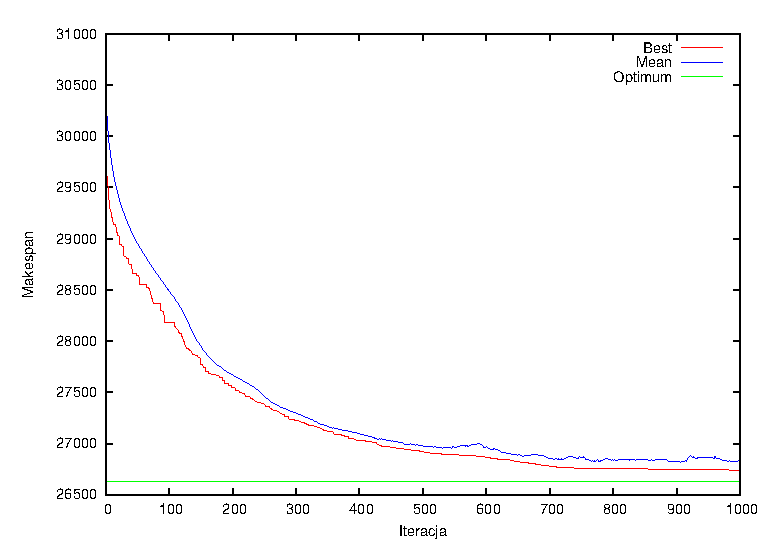
\includegraphics{progres.eps}
\end{center}
\end{figure}

\begin{figure}[H]
\caption{Różnorodność populacji}
\label{diversity}
\begin{center}
  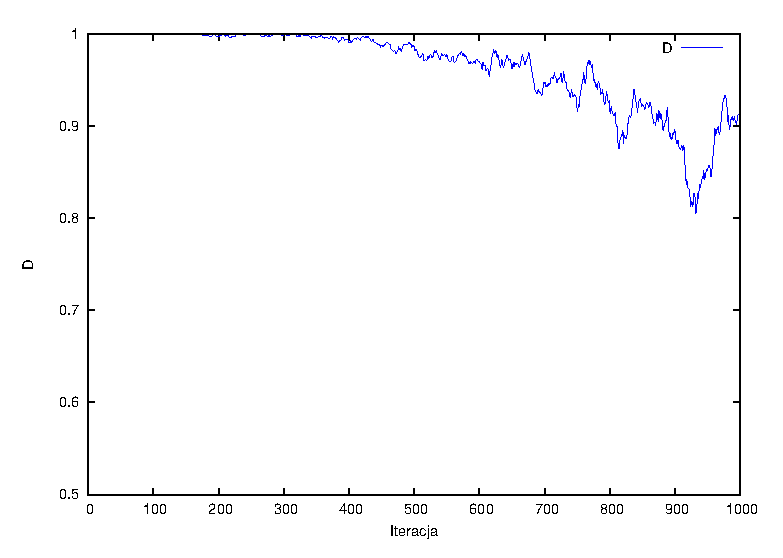
\includegraphics{diversity.eps}
\end{center}
\end{figure}





\section{Wnioski}  
\subsection{Zbieżność algorytmu}
Wykresy \ref{progress}, \ref{diversity} pokazują, że o ile jakość znalezionego rozwiązania z czasem polepsza się 
coraz wolniej, to różnorodność populacji . Oznacza to, że nasz algorytm jest odporny na utykanie
w minimach lokalnych, i nie przestanie działać z powodu zdominowania populacji przez jednego osobnika. Jest to
zasługa strategii zastępowania i losowej imigracji, które chronią różnorodność populacji.

\subsection{Ograniczenia na wielkość problemu}
\subsubsection{Pamięciowe}
W wypadku naszego algorytmu ograniczeniem jest wyłącznie czas jego działania, ponieważ
pamięć zużywana na przechowywanie populacji jest niezmienna w czasie i proporcjonalna do
$n \cdot population\_size$, co nie stanowi żadnego problemu dla współczesnych komputerów.
\subsubsection{Czasowe}
Złożoność pojedynczej iteracji jest zdominowana przez czas przeszukiwania lokalnego, który wynosi
$O(mn^2|Children|)$, zatem złożoność całego algorytmu to $O(smn^2|Children|)$, gdzie $s$ to ilość iteracji.
Trudno powiedzieć, jaka jest górna granica rozmiaru rozwiązywalnego problemu, ponieważ przeszukiwanie 
lokalne jest zaimplementowane równolegle, czyli stała ukryta w notacji $O$ jest odwrotnie proporcjonalna
do liczby procesorów komputera na którym uruchamiamy algorytm. W tabeli \ref{sredniaiteracja} znajdują się 
średnie czasy wykonania iteracji algorytmu dla 1000 osobników i różnych problemów, na komputerze wyposażonym w:
\begin{itemize}
  \item Procesor Intel i7 $8 \times \text{3.4 GHz}$
  \item 16 GB pamięci RAM
\end{itemize}

\begin{table}[H]
\caption{Średni czas iteracji dla 1000 osobników}
\label{sredniaiteracja}
\begin{center}
\begin{tabular}{|l|l|l|}
  \hline
  n & m & średni czas iteracji \\
  \hline
  500 & 20 & 7.3 s \\
  200 & 20 & 1.27 s \\
  200 & 10 & 0.72 s \\
  100 & 20 & 0.36 s \\
  100 & 10 & 0.18 s \\
  100 & 5 & 0.09 s \\
  \hline
\end{tabular}
\end{center}
\end{table}







\begin{thebibliography}{}
\bibitem{tai90} 
Éric D. Taillard. 
Some efficient heuristic methods for the flow shop sequencing problem. 
European Journal of Operational Research, 47(1):65-74, July 1990.
\href{http://mistic.heig-vd.ch/taillard/articles.dir/Taillard1990.pdf}{pdf}

\bibitem{inst}
\url{http://mistic.heig-vd.ch/taillard/problemes.dir/ordonnancement.dir/ordonnancement.html}

\end{thebibliography}


\end{document}
